
%%%%%%%%%%%%%%%%%%%%%%%%%%%%%%%%%%%%%%%%%%%%%%%%%%%%%%%%%%%%%%%%%%%%%%%%%%%%%%%%%%%%%%%
%%%%%%%%%%%%%%%%%%%%%%%%%%%%%%%%%%%%%%%%%%%%%%%%%%%%%%%%%%%%%%%%%%%%%%%%%%%%%%%%%%%%%%%
% 
% This top part of the document is called the 'preamble'.  Modify it with caution!
%
% The real document starts below where it says 'The main document starts here'.

\documentclass[12pt]{article}

\usepackage{amssymb,amsmath,amsthm}
\usepackage[top=1in, bottom=1in, left=1.25in, right=1.25in]{geometry}
\usepackage{fancyhdr}
\usepackage{enumerate}
\usepackage{listings}
\usepackage{graphicx}
\usepackage{float}
% Comment the following line to use TeX's default font of Computer Modern.

\usepackage{times,txfonts}



\makeatletter
\renewcommand*\env@matrix[1][*\c@MaxMatrixCols c]{%
  \hskip -\arraycolsep
  \let\@ifnextchar\new@ifnextchar
  \array{#1}}
\makeatother

\newtheoremstyle{homework}% name of the style to be used
  {18pt}% measure of space to leave above the theorem. E.g.: 3pt
  {12pt}% measure of space to leave below the theorem. E.g.: 3pt
  {}% name of font to use in the body of the theorem
  {}% measure of space to indent
  {\bfseries}% name of head font
  {:}% punctuation between head and body
  {2ex}% space after theorem head; " " = normal interword space
  {}% Manually specify head
\theoremstyle{homework} 

% Set up an Exercise environment and a Solution label.
\newtheorem*{exercisecore}{Exercise \@currentlabel}
\newenvironment{exercise}[1]
{\def\@currentlabel{#1}\exercisecore}
{\endexercisecore}

\newcommand{\localhead}[1]{\par\smallskip\noindent\textbf{#1}\nobreak\\}%
\newcommand\solution{\localhead{Solution:}}

%%%%%%%%%%%%%%%%%%%%%%%%%%%%%%%%%%%%%%%%%%%%%%%%%%%%%%%%%%%%%%%%%%%%%%%%
%
% Stuff for getting the name/document date/title across the header
\makeatletter
\RequirePackage{fancyhdr}
\pagestyle{fancy}
\fancyfoot[C]{\ifnum \value{page} > 1\relax\thepage\fi}
\fancyhead[L]{\ifx\@doclabel\@empty\else\@doclabel\fi}
\fancyhead[C]{\ifx\@docdate\@empty\else\@docdate\fi}
\fancyhead[R]{\ifx\@docauthor\@empty\else\@docauthor\fi}
\headheight 15pt

\def\doclabel#1{\gdef\@doclabel{#1}}
\doclabel{Use {\tt\textbackslash doclabel\{MY LABEL\}}.}
\def\docdate#1{\gdef\@docdate{#1}}
\docdate{Use {\tt\textbackslash docdate\{MY DATE\}}.}
\def\docauthor#1{\gdef\@docauthor{#1}}
\docauthor{Use {\tt\textbackslash docauthor\{MY NAME\}}.}
\makeatother

% Shortcuts for blackboard bold number sets (reals, integers, etc.)
\newcommand{\Reals}{\ensuremath{\mathbb R}}
\newcommand{\Nats}{\ensuremath{\mathbb N}}
\newcommand{\Ints}{\ensuremath{\mathbb Z}}
\newcommand{\Rats}{\ensuremath{\mathbb Q}}
\newcommand{\Cplx}{\ensuremath{\mathbb C}}
%% Some equivalents that some people may prefer.
\let\RR\Reals
\let\NN\Nats
\let\II\Ints
\let\CC\Cplx

%%%%%%%%%%%%%%%%%%%%%%%%%%%%%%%%%%%%%%%%%%%%%%%%%%%%%%%%%%%%%%%%%%%%%%%%%%%%%%%%%%%%%%%
%%%%%%%%%%%%%%%%%%%%%%%%%%%%%%%%%%%%%%%%%%%%%%%%%%%%%%%%%%%%%%%%%%%%%%%%%%%%%%%%%%%%%%%
% 
% The main document start here.

% The following commands set up the material that appears in the header.
\doclabel{STAT 402: Homework 5}
\docauthor{Stefano Fochesatto}
\docdate{\today}


%\textbf{Code:}
%\begin{center}
 %   \lstinputlisting{r1.txt}
%\end{center}

\begin{document}

\begin{exercise}{1} We have aerial counts of bird nests from all $N = 1000$ plots that we 
have divided a region into. The total aerial count is $\tau_x = 4500$. We select a SRS of
size $n = 10$ plots and visit them, performing a very careful 'ground truth' survey.\\

\textbf{The results are:}
\begin{center}
   \lstinputlisting{r1.txt}
\end{center}

\begin{enumerate}
  \item[a.] Find a 95 percent confidence interval for $R$, the ratio of ground count to aerial
   count (this is the reciprocal of the detection probability).\\
   \solution Recall that the estimator for the ratio of random variables $R$ is given by, 
   \begin{equation*}
     \hat{R} = \dfrac{\bar{y}}{\bar{x}}.
   \end{equation*}
   With a variance of, 
   \begin{equation*}
    \hat{V}(\hat{R}) = \dfrac{N - n}{N}\dfrac{1}{\mu^2_x}\dfrac{MSE_R}{n}.
   \end{equation*}
   Computing the 95 percent confidence interval get, \\
   \textbf{Code:}
    \begin{center}
   \lstinputlisting{r2.txt}
    \end{center}
    \vspace{.15in}

  \item[b.] Find a 95 percent confidence interval for $\tau_y$, the total number of nests in the region.\\
  \solution Recall that we can estimate $\tau_y$ by the following formula, 
  \begin{equation*}
    \hat{\tau}_y = \tau_x \dfrac{\bar{y}}{\bar{x}} = \tau_x \hat{R}
  \end{equation*}
  The variance can also be estimated with the following, 
  \begin{equation*}
    \hat{V}( \hat{\tau}_y) = N^2\dfrac{N - n}{N}\dfrac{MSE_R}{n}.
  \end{equation*}
  Computing the 95 percent confidence interval for $\hat{\tau}_y$ we get, \\
  \textbf{Code:}
  \begin{center}
 \lstinputlisting{r3.txt}
  \end{center}
  \vspace{.15in}

   \item[c.] BONUS: Find a 95 percent confidence interval for $1/\tau_y$.

\end{enumerate}
\end{exercise}

\vspace{1in}

\begin{exercise}{2.} If we want to estimate the number of grass blades in a plot, and the plot varies a lot
  in grass density, we might try a rank set sample.  Suppose we can't stand to count more than 4 quadrats
  (of 1 square inch each), and we think that we should be able to easily rank two samples just by looking
  at them.  Describe how I would conduct a rank set sample in this situation (hint:  we'll end up looking
  at 8 quadrats).\\

  In an earlier assignment (Problem 5 in HW 3), you had a number of plots, where you had a guess at the 
  grass cover at all locations (column ‘Guess at Cover’), basically a census for a simple-to-assign variable. 
  In that problem we used the guesses to stratify the population. We could, instead, just collect a SRS 
  and use ratio estimation to get an improved estimate of cover everywhere.\\
  
  You know the guess at grass cover for all the plots:
  \begin{center}
    \lstinputlisting{r4.txt}
  \end{center}

  \begin{enumerate}
    \item[a.] Take a simple random sample of size $n=8$ from the population of plots. In real life 
    you would then go to those plots and measure the true grass cover $Y$. In this assignment 
    you should instead go to the earlier problem (PROBLEM 5 in HW 3) and get the $Y$ values.  
    Then obtain a 95 percent confidence interval for the **mean** grass cover using the ratio 
    estimator approach.\\
    \solution Going back to the data from homework 3, we can conduct a SRS $n = 8$ on the 
    true grass cover, and obtaining a mean grass cover estimator using the ratio estimator.\\
    \textbf{Code:}
    \begin{center}
   \lstinputlisting{r5.txt}
    \end{center}
    \vspace{.15in}

    \item[b.]In a tragic accident, your research assistant lost all of the ‘guess’ measurements. 
    Repeat the analysis using only the 'true cover' values from your sample and the usual 95 percent 
    confidence interval for the mean based on a SRS.\\
    \textbf{Code:}
    \begin{center}
   \lstinputlisting{r6.txt}
    \end{center}
    \vspace{.15in}

    \item[c.]The true average cover is 0.46. Did both of your intervals contain the true average? 
    How do the two intervals compare in width?\\
    \solution The second analysis, which estimated the mean guess cover ended up not containing the 
    true average cover. The confidence interval was shifted down when we used the estimated mean guess cover
    so it must be that our samples skewed lower than the true mean. 
  \end{enumerate}
\end{exercise}
\vspace{1in}


\begin{exercise}{3.} Using the sample from problem 2, compute a 95 percent confidence interval for the mean 
  using the regression estimator. How does it compare to the other approaches?\\
  \solution 
  \textbf{Code:}
  \begin{center}
 \lstinputlisting{r7.txt}
  \end{center}
  The regression estimator introduces a little more variance than either ratio estimator. I do think that the regression 
  estimator is slightly more centered around the true mean, that we know from the data to be around .46 which is almost exactly
  our estimate of the mean. 
\end{exercise}
\vspace{1in}


\begin{exercise}{4.} Sometimes you can transform data to get a better estimate. Suppose there are $N = 200$ 
  plots, and you take an inexpensive estimate of contaminate level in all plots (the is $X$). You also can 
  sample $n = 30$ plots and take a highly accurate measurement $Y$. Unfortunately, the relationship is not 
  linear. Here is the pertinent information:\\
  \textbf{All X values in parts per thousand (inexpensive estimate):}
  \begin{center}
 \lstinputlisting{r8.txt}
  \end{center}
  \textbf{I drew a SRS from this population and also collected the corresponding $Y$ value:}
  \begin{center}
 \lstinputlisting{r9.txt}
  \end{center}
  \begin{enumerate}
    \item[a.] Plot $x_samp$ vs $y_samp$. It is not really linear. Can you find a transformation 
    of $X$ that makes the plot more linear? Apply it and then plot the result.\\
    \solution Plotting the data we get the following, and transforming the $x_samp$ data 
    by squaring it we actually get a higher correlation. The original data gets a correlation of 
    $0.9260864$ and the transformed data get $0.9307337$.
    \begin{figure}[H]
      \begin{center}
      \caption{Plotted Data}
      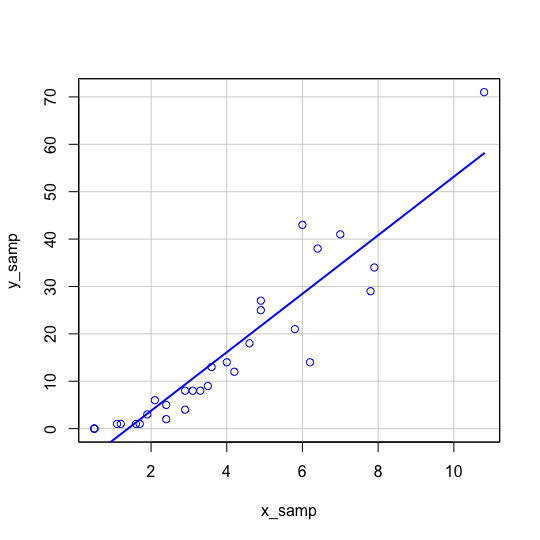
\includegraphics[width=.63\textwidth]{Rplot1.png}
      \end{center}
  \end{figure}
  \begin{figure}[H]
    \begin{center}
    \caption{Transformed Data(Squaring X)}
    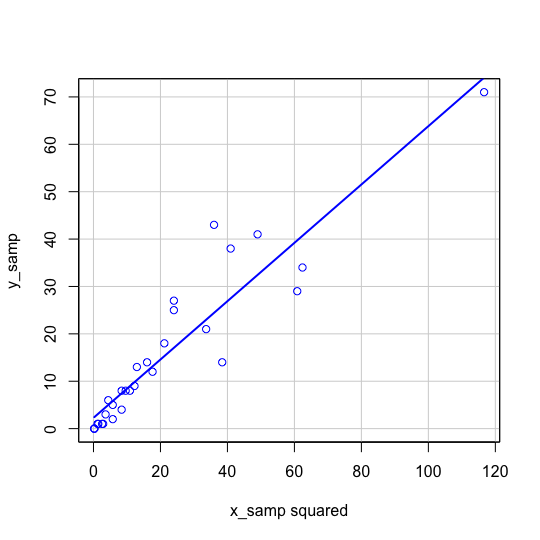
\includegraphics[width=.63\textwidth]{Rplot2.png}
    \end{center}
\end{figure}
    
  \textbf{Code:}
  \begin{center}
 \lstinputlisting{r10.txt}
  \end{center}
  \vspace{.15in}

  \item[b.] Apply this transformation to all of the $X$ values to find the new (transformed) 
  $\tau_{x*}$. Now use either the ratio or regression estimator (your choice) to get a 95 
  percent confidence interval for the average contaminant level in the area.\\
  \solution Applying the ratio estimator on the transformed data, we get
  \textbf{Code:}
  \begin{center}
    \lstinputlisting{r11.txt}
  \end{center}
  Applying a linear model to the transformed data we get an intercept of around -8 with very 
  high significance. That tells me that we will likely get a more accurate estimator for the mean 
  containment level. Doing so we get, \\
  \textbf{Code:}
  \begin{center}
    \lstinputlisting{r12.txt}
  \end{center}



\end{enumerate}

\end{exercise}


\end{document}




















